%--------------------------------------------------
% 1 rate of change
%--------------------------------------------------

\subsection{Exercises 5.2.1}
\begin{enumerate}
\item Find the equation of the tangent line to the parabola $y =x^{2} +4$ at the point $(1 ,5)$. \end{enumerate}


%---------------------------------------------------
% 2 Derivatives from 1st Principles
%---------------------------------------------------

\subsection{Exercises 5.3}
\begin{enumerate}
	\item Find the derivative of the function $f (x) =5 x^{2} +3 x -1$ at the number $2$. 
	
	\item Find the derivative of the function $f (x) =1 -3 x^{2}$ at the number $2$. 
	
	\item Find the derivative of the function $f (x) =x^{4}$ at the number $1$, given
	\begin{equation*}(x +h)^{4} =x^{4} +4 x^{3} h +6 x^{2} h^{2} +4 x h^{3} +h^{4}
	\end{equation*}
	
	\item Find the derivative of the function $F (x) =\sqrt{x}$ at the number $4$ Hint: rationalise the numerator \end{enumerate}

%------------------------------------------------------

\subsection{Worksheet on Sketching Derived Functions}
The graph of $f (x) =(x -1) (x +2) (x -3)$ is drawn below. On the same set of axes, sketch the graph of the derived function, $f^{ \prime } (x)$\vspace{0.5cm} 


\setlength\fboxrule{0.01in}\setlength\fboxsep{0.2in}\fcolorbox[HTML]{000000}{FFFFFF}{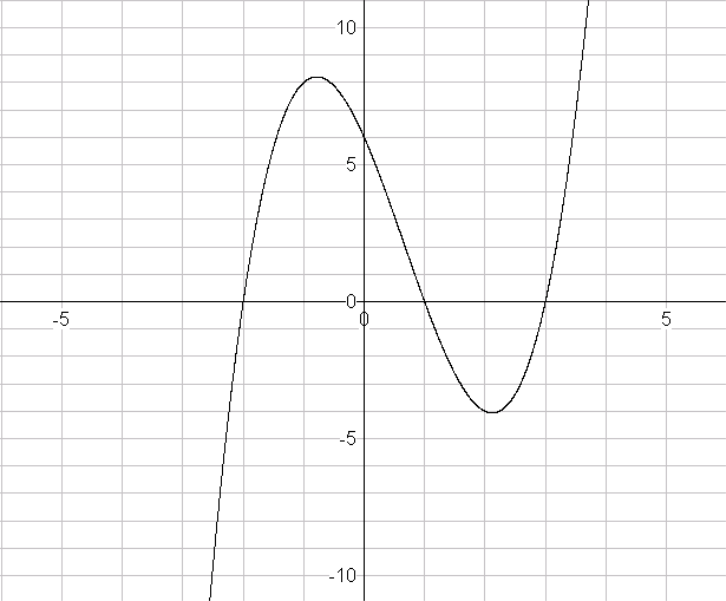
\includegraphics[ width=3.5526in, height=2.9473in,]{L4SZ2834}
}
\vspace{0.5cm} 

What is the shape of the graph of the derived function? 

The graph of $f (x) =(x +1) (x -1) (x -2) (x +3)$ is drawn below. On the same set of axes, sketch the graph of the derived function, $f^{ \prime } (x)\vspace{+0.500000cm}$ 


\setlength\fboxrule{0.01in}\setlength\fboxsep{0.2in}\fcolorbox[HTML]{000000}{FFFFFF}{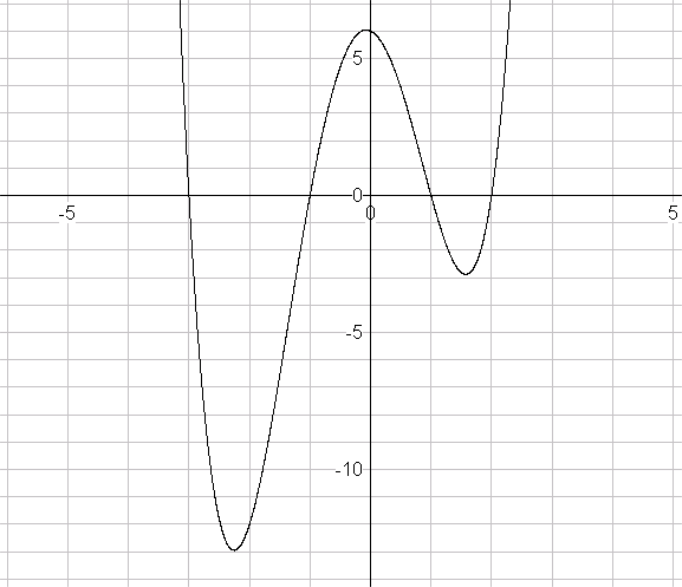
\includegraphics[ width=3.3633in, height=2.9014in,]{L4SZ2835}
}
\vspace{0.5cm}\vspace{0.5cm} 

What
is the order of $f (x)$? \vspace{0.5cm} 

What is the order of $f^{ \prime } (x)$?\vspace{0.5cm} 

The
graph of $f (x) =e^{x}$ is drawn below. On the same set of axes, sketch the graph of the derived function, $f^{ \prime } (x)\vspace{+0.500000cm}$ 


\setlength\fboxrule{0.01in}\setlength\fboxsep{0.2in}\fcolorbox[HTML]{000000}{FFFFFF}{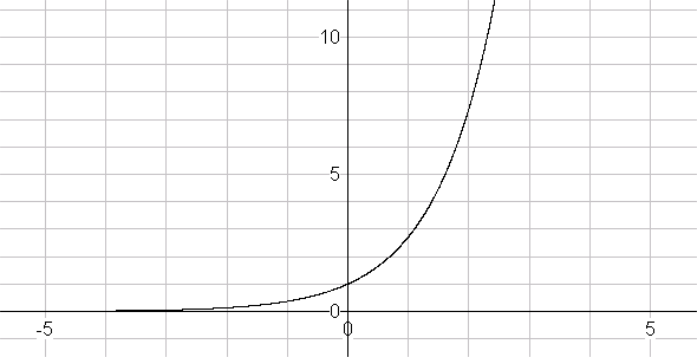
\includegraphics[ width=4.7167in, height=2.4275in,]{L4SZ2836}
}
\vspace{0.5cm} 

What is the shape of the graph of the derived function?\vspace{1cm}


The graph of $f (x) =10 x^{2} e^{x} (x +1)$is drawn below. On the same set of axes, sketch the graph of the derived function, $f^{ \prime } (x)\vspace{+0.500000cm}$ 


\setlength\fboxrule{0.01in}\setlength\fboxsep{0.2in}\fcolorbox[HTML]{000000}{FFFFFF}{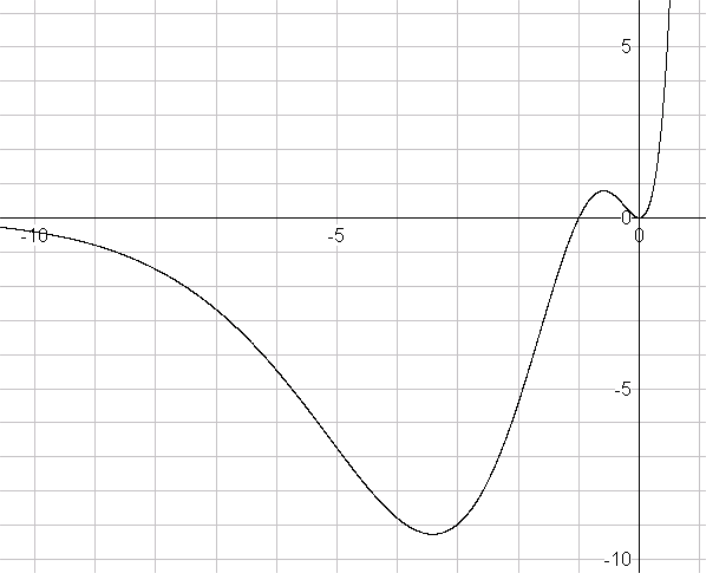
\includegraphics[ width=4.2851in, height=3.4826in,]{L4SZ2837}
}


\subsection{Exercises 5.5.1}
\begin{enumerate}
	\item Differentiate 
	
	
	\begin{enumerate}
		\item $f (x) =\frac{1}{x^{2}}$ 
		
		\item $y =\sqrt[{3}]{x^{2}}$ \end{enumerate}
	
% MOVE TO TANGENTS	
	\item Find the equations of the
	tangent line and the normal line to the curve $y =x \sqrt{x}$ at the point $(1 ,1)$. \end{enumerate}


\subsubsection{Supplementary Exercises}
Differentiate the following expressions for $y$ with respect to $x$.  
%TCIMACRO{\TeXButton{Start 2 Cols}{\columnsep =30pt
% \begin {multicols}{2}}}%
%BeginExpansion
\columnsep =30pt
\begin {multicols}{2}
%EndExpansion



\begin{enumerate}
	\item $y =x^{5}$ 
	
	\item $y =\frac{1}{x^{3}}$ 
	
	\item $y =x^{ -4}$ 
	
	\item $y =x^{3/4}$ 
	
	\item $y =\frac{1}{\sqrt{x}}$ \end{enumerate}



%TCIMACRO{\TeXButton{Stop 2 Cols}{\end {multicols}}}%
%BeginExpansion
\end {multicols}
%EndExpansion

\subsection{Exercises 5.5.3 and 5.5.4}
\begin{enumerate}
	\item Differentiate $x^{8} +12 x^{5} -4 x^{4} +10 x^{3} -6 x +5$ 
	
	\item Find the points on the curve $y =x^{4} -6 x^{2} +4$ where the tangent line is horizontal. \end{enumerate}


\subsubsection{Supplementary Exercises}
\columnsep=30pt
\begin{multicols}{2}
	
	\begin{enumerate}
		\item Differentiate 
		
		
		\begin{enumerate}
			\item $y =\frac{2}{5} x^{5}$ 
			
			\item $y = -10$ 
			
			\item $y = -3 x^{4}$ 
			
			\item $y =\frac{2}{x^{4}}$ 
			
			\item $y =\frac{1}{3 x^{3}}$ \end{enumerate}
		
		
		\item Differentiate 
		
		
		\begin{enumerate}
			\item $f (t) =\sqrt{t}$ 
			
			\item $f (t) =\sqrt{t^{3}}$ 
			
			\item $f (z) =\sqrt[{3}]{z^{5}}$ 
			
			\item $f (x) =2 x^{3.2}$ \end{enumerate}
		
		
		\item Differentiate 
		
		
		\begin{enumerate}
			\item $f (x) =2 x^{3} -3 x^{2} +4 x -1$ 
			
			\item $f (x) =x^{2} +x +1 +\frac{1}{x}$ \end{enumerate}
		
		
		\item Given $s =4 t^{2} -7 t +5$ find $\frac{d s}{d t}$ 
		
		\item Find $\frac{d \left (3 x\right )}{d x}$ 
		
		\item Find $\frac{d \left (3 u^{4}\right )}{d u}$ 
		
		\item Given $f (x) =2 x -3$ find $D f (x)$ \end{enumerate}
\end{multicols}


\subsection{Exercises 5.6.2}
\begin{enumerate}
	\item Given $f (x) =e^{x} -x$ find $f^{ \prime } (x)$. Sketch the graph. 
	
	\item A
	what point on the curve $y =e^{x}$ is the tangent line parallel to the line $y =2 x$? \end{enumerate}


\subsubsection{Supplementary Exercises}
\begin{enumerate}
	\item Find a point $a$ on the curve $f (x) =x^{3} +2 x^{2} +3 x +4$ where $f^{ \prime } (a) =2$. 
	
	\item Differentiate $f (x) =\left (3 x\right )^{3}$. 
	
	\item Differentiate $g (x) =\left (x^{3}\right )^{5}$ 
	
	\item Find the derivative of $f (x) =e^{x} -x^{e}$. 
	
	\item Find where the tangent line to the function $f (x) =x^{3} -x +1$ is parallel to the line $y =x$. 
	
	\item Differentiate $f (x) =\frac{1}{x^{3}} -\frac{1}{\sqrt[{4}]{x^{3}}}$. 
	
	\item Differentiate $f (x) =\frac{\sqrt{x} +\sqrt[{3}]{x}}{\sqrt[{4}]{x}}$. 
	
	\item Find the derived function of $g (x) =e x^{2} +2 e^{x} +x e^{2} +x^{e^{2}}$ 
	
	\item Find the derivative of $f (x) =\sqrt[{3}]{x} +\sqrt[{5}]{2}$. \end{enumerate}


\subsection{Exercises 5.7.1}
\begin{enumerate}
	\item If $f (x) =x e^{x}$ find $f^{ \prime } (x)$. 
	
	\item Find the derivative of $g (x) =x^{2} e^{x}$. 
	
	\item If $y =\left (r^{2} -2 r\right ) e^{r}$ find $\frac{d y}{d r}$. \end{enumerate}


\subsubsection{Supplementary Exercises}
Differentiate with respect to $x$ 


\begin{enumerate}
	\item $x^{3} e^{x}$ 
	
	\item $x^{ -3} e^{x}$ 
	
	\item $\left (x +1\right ) e^{x}$ 
	
	\item $\left (x +2\right ) \left (x -2\right ) e^{x}$ \end{enumerate}


\subsection{Exercises 5.7.2}
\begin{enumerate}
	\item Given $y =\frac{3 x +1}{2 x -1}$ find $y^{ \prime }$. 
	
	\item Differentiate $y =\frac{e^{x}}{x +1}$. 
	
	\item If $f (t) =\frac{2 t}{1 +t^{2}}$ find $\frac{d f}{d t}$. 
	
	\item Find the derived function for $f (x) =\frac{A}{B +C e^{x}}$. \end{enumerate}


\subsubsection{Supplementary Exercises}
Differentiate 


\begin{enumerate}
	\item $\frac{3 x^{2}}{1 -x}$ 
	
	\item $\frac{x}{x +2}$ 
	
	\item $\frac{\sqrt{x}}{x +2}$ 
	
	\item $\frac{2 x^{2} +3 x +2}{e^{x}}$ \end{enumerate}


\subsection{5.7.3 Exercises involving Tangent and Normals}
\begin{enumerate}
	\item Find the equation of the tangent line and normal line to the curve $y =x e^{x}$ at the point $\left (0 ,0\right )$ 
	
	\item The
	curve $y =1/(1 +x^{2})$ has the name \textbf{witch of Maria Agnesi.} 
	
	
	\begin{description}
		\item [(a)] Find the equation of the tangent line to this curve at the point
		$\left (1 ,\frac{1}{2}\right )$. 
		
		\item [(b)]
		Use Desmos to draw the graph of the curve and the tangent line on the same grid. \end{description}
	
	\item The
	curve $y =x/(1 +x^{2})$ is called a \textbf{serpentine}. 
	
	
	\begin{description}
		\item [(a)] Find the equation of the tangent line at the point $\left (1 ,\frac{1}{2}\right )$. 
		
		\item [(b)]
		Use Desmos to draw the graph of the curve and the tangent line on the same grid. \end{description}\end{enumerate}


\subsection{Exercises 5.8.1}
\begin{enumerate}
	\item Let $f (x) =\sqrt{x}$ and $g (x) =x^{3}$ find $\left (f \circ g\right ) (x)$ and $\left (g \circ f\right ) \left (x\right )$. 
	
	\item Given $h \left (x\right ) =e^{x}$ and $j (x) =\frac{x^{2}}{2}$ find $\left (h \circ j\right ) (x)$ and $\left (j \circ h\right ) (x)$. \end{enumerate}


\subsection{Exercises 5.8.5}
\begin{enumerate}
	\item   
	%TCIMACRO{\TeXButton{Start 2 Cols}{\columnsep =30pt
	% \begin {multicols}{2}}}%
	%BeginExpansion
	\columnsep =30pt
	\begin {multicols}{2}
	%EndExpansion
	Find $F^{ \prime } (x)$ when $F (x) =\sqrt{1 +x^{2}}$. 
	
	\item Given $y =\left (1 -x^{2}\right )^{5}$ find $\frac{d y}{d x}$. 
	
	\item Find the derivative of $e^{x^{2}}$. 
	
	\item Find the derived function for $e^{e^{x}}$. 
	%TCIMACRO{\TeXButton{Stop 2 Cols}{\end {multicols}}}%
	%BeginExpansion
	\end {multicols}
	%EndExpansion
\end{enumerate}


\subsubsection{Supplementary Exercises}
Differentiate with respect to $x$ 


\begin{enumerate}
	\item   
	%TCIMACRO{\TeXButton{Start 2 Cols}{\columnsep =30pt
	% \begin {multicols}{2}}}%
	%BeginExpansion
	\columnsep =30pt
	\begin {multicols}{2}
	%EndExpansion
	$\left (3 x +2\right )^{3}$ 
	
	\item $\left (4 -3 x\right )^{3}$ 
	
	\item $\left (5 x +3\right )^{\frac{3}{5}}$ 
	
	\item $\frac{1}{2 x +1}$ 
	
	\item $\frac{3}{\left (4 -x\right )^{3}}$ 
	
	\item $\sqrt{2 x -5}$ 
	
	\item $\sqrt[{3}]{5 -x^{2}}$ 
	
	\item $\frac{1}{\sqrt{x +2}}$ 
	
	\item $e^{2 x^{3}}$ 
	%TCIMACRO{\TeXButton{Stop 2 Cols}{\end {multicols}}}%
	%BeginExpansion
	\end {multicols}
	%EndExpansion
\end{enumerate}

\subsection{Exercises 5.9}
\begin{enumerate}
	\item Given $y =x^{2} e^{ -2 x}$ find $\frac{d y}{d x}$ 
	
	\item Differentiate $\left (1 -2 x\right )^{2} e^{ -x}$ 
	
	\item Find the derivative of $\frac{p +1}{\sqrt{p^{2} +1}}$. \end{enumerate}


\subsubsection{Supplementary Exercises}
Differentiate 


\begin{enumerate}
	\item   
	%TCIMACRO{\TeXButton{Start 2 Cols}{\columnsep =30pt
	% \begin {multicols}{2}}}%
	%BeginExpansion
	\columnsep =30pt
	\begin {multicols}{2}
	%EndExpansion
	$\left (x^{2} +3\right )^{2} \left (x -4\right )$ 
	
	\item $\left (x -3\right )^{3} \left (x +2\right )$ 
	
	\item $\sqrt{x +1} \left (x -1\right )^{2}$ 
	
	\item $e^{x^{2}} \sqrt{x +1}$ 
	
	\item $\frac{x^{2} +x +2}{\left (x +1\right )^{2}}$ 
	
	\item $\frac{\left (x -3\right )^{3}}{\left (x +2\right )}$ 
	%TCIMACRO{\TeXButton{Stop 2 Cols}{\end {multicols}}}%
	%BeginExpansion
	\end {multicols}
	%EndExpansion
\end{enumerate}

\subsection{Exercises 5.10.1}
\begin{enumerate}
	\item Sketch the graph of 
	
	
	\begin{enumerate}
		\item $f (x) =\sin  x$ 
		
		\item $g (x) =\cos  x$ 
		
		\item $h (x) =\tan  x$ \end{enumerate}
	
	
	\item Sketch the graph of $f^{ \prime } (x)$ where $f (x) =\sin  x$ 
	
	\item Sketch the graph of $g^{ \prime } (x)$ where $g (x) =\cos  x$ \end{enumerate}


\subsection{Exercises 5.10.2 (a)}
\begin{enumerate}
	\item Verify that $\tan  x =\frac{\sin  x}{\cos  x}$ 
	
	\item Use the trigonometric identity $\tan  x =\frac{\sin  x}{\cos  x}$ and the \emph{Quotient Rule }to show the derivative of $h (x) =\tan  x$ is $h^{ \prime } (x) =\sec ^{2} x$ \end{enumerate}




\subsection{Exercises 5.10.2 (b)}
\begin{enumerate}
	\item [3.] Differentiate $y =x^{2} \sin  x$ 
	
	\item [4.] Differentiate $f (x) =\sqrt{x} \sin  x$ 
	
	\item [5.] Differentiate $h (x) =\tan  (5 x)$ 
	
	\item [6.] Differentiate $y =\frac{x}{\cos  x}$ 
	
	\item [7.] Differentiate $g (t) =\cos  (\omega  t +\delta )$ 
	
	\item [8.] Find the tangent line to the curve $y =e^{x} \cos  x$ at the point $(0 ,1)$. 
	
	\item [9.]
	A ladder $10 \mbox{m}$ long rests against a vertical wall. Let
	$\theta $ be the angle between the top of the ladder and the wall and let $x$ be the distance between the bottom of the ladder and the wall. If the bottom of
	the ladder slides away from the wall, how fast is $x$ changing with respect to $\theta $ when $\theta  =\frac{\pi }{3}$? \end{enumerate}


\subsubsection{Supplementary Exercises}
Differentiate 


\begin{enumerate}
	
	%TCIMACRO{\TeXButton{Start 2 Cols}{\columnsep =30pt
	% \begin {multicols}{2}}}%
	%BeginExpansion
	\columnsep =30pt
	\begin {multicols}{2}\item
	%EndExpansion
	$\sin  4 x$ 
	
	\item $\frac{2}{\pi } \sin  \pi  x$ 
	
	\item $5 \sin  \left (x +\frac{\pi }{4}\right )$ 
	
	\item $5 \cos  3 x$ 
	
	\item $12 \cos  \left (\frac{\pi }{2} -3 x\right )$ 
	
	\item $\tan  3 x$ 
	
	\item $3 \tan  \left (x +2\right )$ 
	
	\item $\sin ^{3} x$ 
	
	\item $\sin ^{2} 3 x$ 
	
	\item $\sin ^{3} \left (x -1\right )^{2}$ 
	
	\item $\cos ^{2} \left (\pi  -x\right )^{2}$ 
	
	\item $\tan ^{2} 2 x$ 
	%TCIMACRO{\TeXButton{Stop 2 Cols}{\end {multicols}}}%
	%BeginExpansion
	\end {multicols}
	%EndExpansion
\end{enumerate}




\subsection{Exercises 5.11 (a)}
\begin{enumerate}
	\item If $f (x) =2 x^{2} -x^{3}$find $f^{ \prime }$, $f^{ \prime  \prime }$, $f^{ \prime  \prime  \prime }$, $f^{(4)}$. 
	
	Use DesmosDesmos to graph $f$, $f^{ \prime }$, $f^{ \prime  \prime }$, and $f^{ \prime  \prime  \prime }$ on a common screen. Describe whether these graphs are consistent with a geometric interpretation
	of these derivatives. 
	
	\item If $f (x) =\frac{1}{x}$ find $f^{ \prime } (x)$ and $f^{ \prime  \prime } (x)$ then graph $f$, $f^{ \prime }$and $f^{ \prime  \prime }$ on a common screen. Are your answers reasonable? \end{enumerate}



\subsection{Exercises 5.11 (b)}
\begin{enumerate}
	\item [3.] Sketch a graph and give its equation for 
	
	
	\begin{enumerate}
		\item a curve whose slope is always positive and increasing. 
		
		\item a
		curve whose slope is always positive and decreasing. \end{enumerate}
	
	
	\item [4.]
	Sketch the graph of a function whose first and second derivatives are always negative. 
	
	\item [5.]
	Sketch the graph of a function whose first derivative is always negative and whose second derivative is always positive. 
	
	\item [6.]
	Sketch the graph of a function that satisfies all of the following conditions
	\begin{align*}f^{ \prime } (0) &  = f^{ \prime } (4) =0 \\
	f^{ \prime } (x) &  >  0\text{ when }x <0 \\
	f^{ \prime } (x) &  < 0\text { if }0 <x <4\text{ or if }x >4 \\
	f^{ \prime  \prime } (x) &  >  0\text{ if }2 <x <4 \\
	f^{ \prime  \prime } (x) &  <  0\text{ if }x <2\text{ or }x >4\end{align*}
	
	\item [7.] Given $f^{ \prime } (x) =x e^{ -x^{2}}$ 
	
	
	\begin{enumerate}
		\item On what interval is $f$ increasing? (Hint: use Desmos) 
		
		\item On what intervals is $f$ decreasing? 
		
		\item Does $f$\ have a local maximum or local minimum? \end{enumerate}
\end{enumerate}


\subsection{Exercises 5.12.1}
Use Desmos to sketch the following parametric curves 


\begin{enumerate}
	\item $x =t^{2} -2 t$ and $y =t +1$ where $0 \leqslant t \leqslant 4$ 
	
	\item $x =\cos  t$ and $y =\sin  t$ where $0 \leqslant t \leqslant 2 \pi $ 
	
	\item $x =2 \cos  t$ and $y =\sin  t$ where $0 \leqslant t \leqslant 2 \pi $ 
	
	\item $x =\cos  t$ and $y =\sin  2 t$ where $0 \leqslant t \leqslant 2 \pi $ 
	
	\item $x =1.5 \cos  t -\cos  40 t$ and $y =1.5 \sin  t -\sin  40 t$ where $0 \leqslant t \leqslant 2 \pi $ \end{enumerate}




\subsection{Exercises 5.12.2}
\begin{enumerate}
	\item Given $y =2 t$ and $x =t^{2}$ 
	
	
	\begin{enumerate}
		\item Find $\frac{d y}{d x}$. 
		
		\item By finding the appropriate value of $t$ show that $(1 ,2)$ lies on the parametric curve. 
		
		\item Find
		the equation of the tangent line to the parametric curve at $(1 ,2)$. \end{enumerate}
	
	
	\item Given
	$x =\cos  t$ and $y =\sin  t$ find the equation of the tangent line at the point $\left (\frac{\sqrt{2}}{2} ,\frac{\sqrt{2}}{2}\right )$. Where does this curve
	have horizontal or vertical tangent lines? 
	
	\item Given $x =\cos  t$ and $y =\sin  2 t$ find the equation of the tangent line at the point $\left (\frac{\sqrt{3}}{2} ,\frac{\sqrt{3}}{2}\right )$. Where does this curve
	have horizontal or vertical tangent lines? \end{enumerate}


\subsubsection{Supplementary Exercises}
Find $\frac{d y}{d x}$ in terms of the parameter 


\begin{enumerate}
	
	
	\columnsep =30pt
	\begin {multicols}{2}
	\item $x =t^{2} +t\text{\quad \quad }y =t^{3} -t^{2}$ 
	
	\item $x =e^{t} \cos  t\text{\quad \quad }y =e^{t} \sin  t$ 
	
	\item $x =a t^{2}\text{\quad \quad }y =2 a t$ ($a$ is constant) 
	
	\item $x =a \sin  \theta \text{\quad \quad }y =b \cos  \theta $ 
	
	\item $x =2 \sin  \theta \text{\quad \quad }y =\cos  2 \theta $ 
	
	\item $x =a \left (\theta  -\sin  \theta \right )\text{\quad \quad }y =a \left (1 -\cos  \theta \right )$ 
	%TCIMACRO{\TeXButton{Stop 2 Cols}{\end {multicols}}}%
	%BeginExpansion
	\end {multicols}
	%EndExpansion
\end{enumerate}



% related rates exercises
\subsection{Exercises 5.15.1}
\begin{enumerate}
	\item If $V$ is the volume of a cube with edge length $x$ and the cube is expanding as time passes, find $\frac{d V}{d t}$ in terms of $\frac{d x}{d t}$ 
	
	\item Each side of a square is increasing at a rate of $6 \mbox{cm}$/$\mbox{s}$. At what rate is the area of
	the square increasing when the area of the square is $16 cm^{2}$? 
	
	\item  
	
	
	\begin{enumerate}
		\item If $A$ is the area of a circle with radius $r$ and the circle expands as time passes find $\frac{d A}{d t}$ in terms of $\frac{d r}{d t}$ 
		
		\item Suppose oil spills from a ruptured tanker and spreads in a circular pattern.
		\ If the radius of the oil spill increases at a constant rate of $1 \mathrm{m}/\mbox{s}$ how fast is the area of the spill increasing when the radius is $30 \mbox{m}$? \end{enumerate}
	
	
	\item If
	a snowball melts so that its surface area decreases at a rate of $1 cm^{2}$/$\mbox{min}$, find the rate at which the diameter decreases when the diameter is $10$ $\mbox{cm}$. You should use the following steps to solve this
	problem. 
	
	
	\begin{enumerate}
		\item What quantities are given in the problem? 
		
		\item What is
		the unknown? 
		
		\item Draw a picture of the situation for any time $t$. 
		
		\item Write an equation that relates the quantities. 
		
		\item Finish
		solving the problem \end{enumerate}
	
	
	\item At noon ship A is $150 \mbox{km}$ west of a ship B. Ship A is sailing east at $35 \mbox{km}$/$\mbox{h}$ and ship B is sailing north at $25 \mbox{km}$/$\mbox{h}$. How fast is the distance between
	the ships changing at 4:00 P.M.? 
	
	\item A plane flying horizontally at an altitude of $2 \mbox{km}$ and a speed of $800 km/\mbox{h}$ passes directly over a radar station. Find the rate at which the distance from the plane
	to the station is increasing when it is $3 \mbox{km}$ away from the station. \end{enumerate}



\subsection{Exercises 5.15.2}
\begin{enumerate}
	\item Divide $50$ into two parts such that the product of the two parts is a maximum. 
	
	\item Find
	the number that exceeds its square by the greatest amount. 
	
	\item A farmer has $2400 \mbox{m}$ of fencing and wants to fence off a rectangular field that borders a straight
	river. He needs no fence along the river. What are the dimensions
	of the field that has the greatest area? 
	
	\item A farmer wishes to fence off a corner of a field where
	there is an existing hedge on two sides. The hedge is to be used to fence the two sides. If
	he has $300 \mbox{m}$ of fencing available, find the dimensions $a$ and $b$ so that he encloses the maximum area. \\\relax    
	\setlength\fboxrule{0in}\setlength\fboxsep{0.2in}\fcolorbox[HTML]{000000}{FFFFFF}{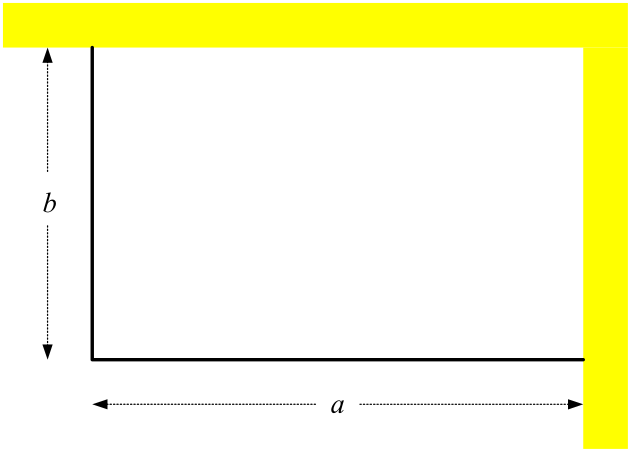
\includegraphics[ width=2.5711in, height=1.8498in,]{L4SZ2838}
	}
	
	
	\item A cylindrical can is to be made to hold $1\,$L of oil. Find the dimensions that will minimise the cost of the
	metal to manufacture the can. (Hint: 1\thinspace L = $1000 cm^{3}$ 
	
	\item Find the area of the greatest rectangle that can be inscribed in a semicircle
	of radius $r$. 
	
	\item If $1200 cm^{2}$ of material is available to make a box with a square base and an open top. Find the largest
	possible volume of the box. (Hint: There is no wasted material.) \end{enumerate}